\chapter{Background}\label{chp:background}


\section{Passwords}
Passwords are the common way of authenticating users upon access to sites on the Internet, the idea is that only the user and the target service knows the password, and the user have to provide the correct password before access are granted. Passwords are a much discussed theme and claiming that passwords are usually not used in the correct manner is not an overreaction. The main problem seems to be the fact that good passwords and the human memory does not go well together. For passwords to be sufficient as authentication each user has to be forced into using long complex password, or even use one generated for them, with the problem being that it is easily forgotten. Further more, if a user was able to memorize \emph{one} "good" password, he will probably use this for all of his accounts, so that if one of the services is compromised and user information leaked, all his accounts may be compromised. With all of this in mind it is easy to say that everybody should use complex, unique passwords for each account, but in practice this is not feasible. Florêncio and Herley ~\cite{password-habits} conducted a large scale study of passwords habits in 2007, revealing that a user on average has 25 different accounts protected by passwords. On average these sites are protected by about 7 distinct password, where 5 of them are rapidly re-used.
\par Password authentication requires the authenticating server to store something related to the password, if this is stolen the password will in most cases be compromised as well, even if the server did not store the clear text password, attackers will, in most cases, be able to retrieve the password eventually. After obtaining the username and password for one service the attacker would try this user data on other services and compromise these as well. 
\par If a user was to have different passwords for each site, these might still easily be compromised. Ives et al. ~\cite{domino-effect} discuss this "domino effect", where intrusion to one domain can compromise several others, if users have re-used passwords.  A normal user will typically try to log in by trial-and-error ~\cite{single-pw-auth}, if the first password does not work, the user will try with another of his passwords. This way may passwords might be lost through phising attacks where a user is tricked into trying to log in to a fake site. It is thus clear that some kind of system is needed to allow a human user to manage strong passwords. The best case would be if each user, for each of his 25 accounts had a unique password of satisfying strength, this is of course not possible.

\subsection{Password strength}\label{password-strength}
How to measure the strength of passwords is a well known and discussed problem, but the general idea is that password strength is related to how strong a password is against brute force attacks. Length and complexity is the most thought of parameters to measure such strength. A perfect password would thus be one as long as allowed by the system consisting of random characters from all possible characters, this one would also be changed frequently. All these characteristics despite how the human brain works. Yan et al.~\cite{memorability_yan} investigate the trade of between security of passwords versus memorability allowing humans to remember them. An important regarding this trade-off is that most sites applying advices and policies on how to create strong passwords, does not take into account if the advices passwords are hard or easy to remember. Point being that there is no point in having a strong password if the user is going to forget it. They suggest that passwords should appear random but be constructed using a  mnemonic structure such ass passphrases. The idea here is to generate a random looking password by memorizing a familiar sentence and using the first letters of each word as the password. Florêncio et al.~\cite{strong-pws_florencio} investigate another matter; do strong passwords accomplish anything? The point being that no matter how long and complex password users chose they are still subject to the most dangerous and common threats (phising, keylogging or access attacks), as discussed in the previous section. The reason for enforcing strong passwords seems to be to protect against bulk guessing attacks, against other attacks, typically offline attacks, shorter passwords is usually sufficient. 

\paragraph{Password strength meters} are a common way used by many sites on the Internet to aid their users when selecting passwords. Common meters use colored progression bars together with a word or short comment stating if the entered password is evaluated as "bad", "poor" or "strong". Ur et al. \cite{password-meters2} found that password meters actually lead users into choosing longer and stronger passwords, but they also argue that enforcing such policies might frustrate users and possibly lead them into writing passwords down, use weak password management schemes or re-use the same password across many sites. The most common requirements used by passwords meters of known web services can be summarized as the following \cite{password-meters}:
\begin{itemize}
    \item{Length and character selection} are part of most password meters. It is normal to disallow passwords shorter, and sometimes longer, than a given range, which may vary. A variation of different characters can be required, namely different kinds of symbols or capital letters. Spaces may be allowed in between other characters, at the start or end of the password, or not at all. Some sites checks for sequences of the same character as well.
    \item{Personal information.} Information registered by the user are evaluated by some meters, typically name, email and date of birth are checked against in original and transformed forms. This means that a password like "4nD3r?1991" ("anders1991" transformed) which look strong, will be evaluated as weak.
    \item{Dictionary checks.} Make sure that the password does not include any dictionary words by matching it with a dictionary of common words. 
\end{itemize}

\paragraph{Entropy}
\todo{write about entropy, \cite{password-policy}}


\par The conclusion on what "good" passwords are, is not clear, but the one thing agreed upon seems to be that re-use of passwords are the biggest threat. It is a fact that the human brain is not capable of remembering different passwords for each account on the Internet, thus the need for an aiding application such as the one discussed in this project. 



\subsection{Attacks}
Passwords are often the only barrier stopping adversaries from directly accessing the accounts of a user. The combination of user name and password are the easiest point of entry to access, and thus the first logical point of attack. There are several methods used to attack password authentication, trying to retrieve passwords. The most important attacks and their respective mitigation technique \cite{nist-guide, strong-pws_florencio}, will be discussed in the following section. 
\paragraph{Capturing} of passwords directly from the server responsible for the authentication involves the attack acquiring password data through breaking into the data storage, eavesdropping on communication channels or through monitoring the user by other means. The first most basic threat are to simply steal the stored password from an insecure server, this would require a weak configured server storing the passwords in plain text. This is mitigated by storing only cryptographic hashes of passwords, which allows the server to authenticate users while preventing attackers from determining the actual passwords without \emph{cracking} the hashes.

\paragraph{Cracking} requires the attacker to go through several steps. First acquiring the hash of a user account or a whole file of hashes for a site. Next, one would try to find a sequence of string yielding the same hash as the actual password. How hard it is to crack a hash depends on the strength of the password and can be mitigated by choosing strong passwords and changing these frequently.\emph{ Rainbow tables }~\cite{rainbow-tables} are a technique employed by attackers to speed up this process. Rainbow tables are precomputed table of hashes, allows the attacker to compute a set of hashes once and use these values several times, thus providing a space-time trade-off. This involves using more space, since all the computed hash values would have to be stored somewhere, but allowing a much shorter computation time to brute-force a hash. The technique stores chains of hashes as shown in figure ~\ref{rainbow-table}, storing only the first and last value of the chain. The attacker then search for a given hash in the set of end points, if no match are found the hash function is applied and a new search conducted. This process continues, until a match is found, the plain text is then then computed from the start value of the chain, applying the hash function the same amount of times it took to find a match in the chain. \todo{rewrite - more precise }



\begin{figure}[h]
    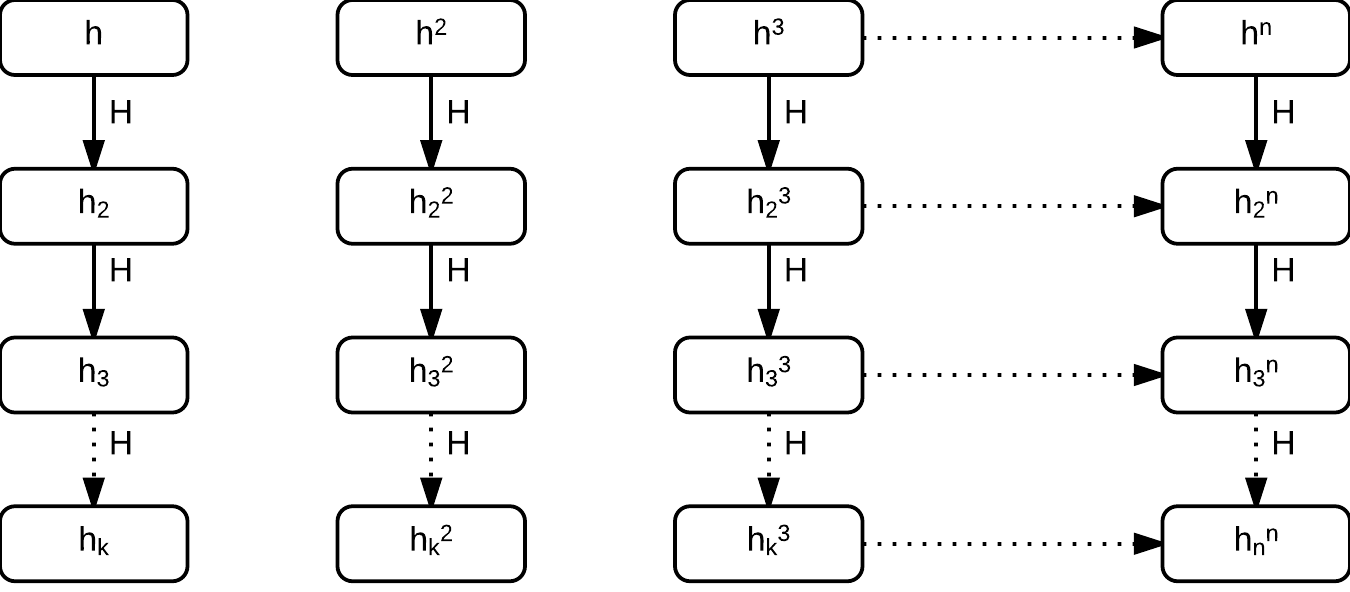
\includegraphics[width=\textwidth]{rainbow-table}
    \caption{Rainbow table}
    \label{rainbow-table}
\end{figure}

%\subsection{Password Storage}

\subsection{Alternative authentication methods}
\todo[inline]{alternative auth: graphical passface etc.}


\section{Human Behavior}
"Good passwords" as discussed in \ref{password-strength} does not go well with the human memory. The first limitation which will be an important property later are the limitation to how much data we can store in immediate memory, this limit was showed to be 7 chunks of data at once~\cite{magic-seven_miller}. This data can not be from a random selection which is what a good password requires.   
\todo[inline]{in progress: human behaviour}





\section{Password Management}
As seen in the previous sections passwords introduce a dilemma as passwords are supposed to be hard to "guess" and thus hard to remember. The naive solution to this problem is to either use one password for many accounts or to write down passwords, even tough most users understand that this solution is bad, users will still do it if the password policy required is too complex.  





\section{Browser Extensions}
Modern computer users shift towards doing more and more work through their web browsers. Web applications have become popular due to the ubiquity of browsers, thus allowing web apps to run anywhere. A web app can run at any platform running a web browser, allowing the application to run on multiple platforms as well as different devices. Updates can be applied quickly without having to distribute patches to a possibly huge amount of devices.
\par Browser extensions add additional features to the web browser allowing the user to tweak the experience of the web pages visited. Typical examples are extensions adding to, or tweaking already present features of the browser such as changing how bookmarks are managed, or adding additional features such as blocking advertisements. Lately browser extensions have been extended even further allowing standalone applications to be developed running as native applications ~\cite{chrome-app-blog}. This allows developers to create desktop apps using the same technology as in web apps, mainly HMTL5, Javascript and CCS.
\par This chapter will present Google chrome browser extensions, including architecture and security mechanisms.

%This project will utilize chrome extensions to create a password manager running in the browser. 
%The user interface will be in a panel spawned by a browser action activated when the user click the icon in the navbar. 
%The user interface is built using the open-source web application framework AngularJS \cite{angularjs}, storage is done using the chrome local storage API.

\subsection{Extension Security}
\par Browser extensions introduce some security concerns which must not be forgotten while developing applications using this environment. Chrome extensions run in the browser with access to both the DOM of the active page as well as the native file system and connected devices. The overall architecture of the application is summarized in \autoref{extension-architecture} and described in the chrome extensions documentation \cite{chrome-extensions}. This section will describe the architecture considering security concerns relevant when developing chrome extensions which handles sensitive data such as passwords.

%The extension core consist of the actual application interface visible to the user as well as long running background jobs and business logic. The background page can be used to spawn panels or popups, and has access to browser APIs.  The extensions is activated through a icon in the browser navbar as seen in \autoref{extension-ux}. Clicking the icon typically spawns a popup or a panel to interact with the user. In addition to the core, each extensions can have content scripts which has access to the content of the current active web page, and can monitor and alter \gls{dom} of this. 


\par Earlier extensions written for IE and Firefox ran in the same process as the browser and shared the same privileges. This made extensions an attractive entry point for attackers, since a buggy extension could leave security holes leaking sensitive information or even provide an entry point to the underlying operating system. For these browsers several frameworks for security have been proposed \cite{firefox-ie, js-info-flow}, trying to mitigate vulnerabilities is browser extensions. The chrome extensions architecture is built from scratch with security in mind, chrome uses a permission system following three principles \cite{liu-chrome}; least privileges, privilege separation and strong isolation. 

\paragraph{Least privileges} specifies that extensions should only have to privileges they need functions, not share those of the browser. The privileges of each extension are requested in the \emph{manifest} file \cite{chrome-manifest}. This json file needs to be included in all chrome extensions, and consist of all the permissions needed by the extension as well as some meta data and version information. This is done to prevent compromised extensions from exploiting other permissions than those available at runtime. An example of a manifest file can look like this: 

\begin{verbatim}
{
    "name": "Example extensions",
    "description": "An example extensions to demonstrate how the
                    manifest file works.",
    "version": "1.2",
    "manifest_version": "2"
    "background_page": "main.hmtl",
    "permissions": [
        "bookmarks",
        "storage",
        "https://*.ntnu.no"
    ]
}
\end{verbatim}
This extension has specified access to the bookmarks API, chrome local storage and all sub domains of ntnu.no. Extensions can request different permissions in the manifest file including web site access, API access and native messaging \cite{chrome-manifest}. If an extension contains weaknesses it will not compromise any other parts of the system not covered by the specified privileges. For the least privileges approach to work properly each developer should only request the permissions needed, Barth et al. \cite{protecting-browsers} examined this behavior and concluded that developers of chrome extensions usually limit the origins requested to the ones needed. 

\paragraph{Privilege separation.} Chrome extensions are as mentioned divided into components; content scripts, extension core and native binaries. The addition of native binaries allows extensions to run arbitrary code on the host computer, thus posing a serious security threat. This project does not use this permission, this component will thus not be mentioned from now on. Content scripts are javascript files allowing extensions to communicate with untrusted web content of the active web page. This scripts are instantiated for each visited web page and has direct access to the \gls{dom} of these, allowing both monitoring and editing of DOM elements. To be able to inject content scripts to a visited page, the origin of the site has to be added to the manifest file. Other than this permission, content script are only allowed to communicate with the extension core. It is important that the privileges of these scripts are at the minimum level since they are at high risk of being attacked by malicious web sites \cite{chrome-extension-dangers}, due to the direct interaction with the \gls{dom}. 
\par The extension core is the application interface responsible for interaction with the user as well as long running background jobs and business logic. The core is written in HTML and javascript and are responsible for spawning popups and panels, as well as listening for browser action. The typical way to activate a extensions is by clicking a icon in the navigation bar, which then activates either a popup or a detached panel. The core is the components with the most privileges as it does not interact with any insecure content directly, only through direct messaging to a content script or using http requests if the target origin is defined in the manifest. In addition to this the core has access to the extension APIs, these are special-purpose interfaces providing additional features such as alarms, bookmarks, cookie and file storage. The APIs are made available through the manifest file and only those specified there can be used. \autoref{extension-ux} illustrates the interaction between the background page, content scripts, panels and active web page. The information flow starts by clicking the extension's icon in the navigation bar which launch the background page spawning a panel in the browser. A content script is injected in the current web site (google.no in the example), the script now have access to the DOM of this site and can communicate with the background which in turn can update the panel. 


\begin{figure}[h]
    \fbox{ 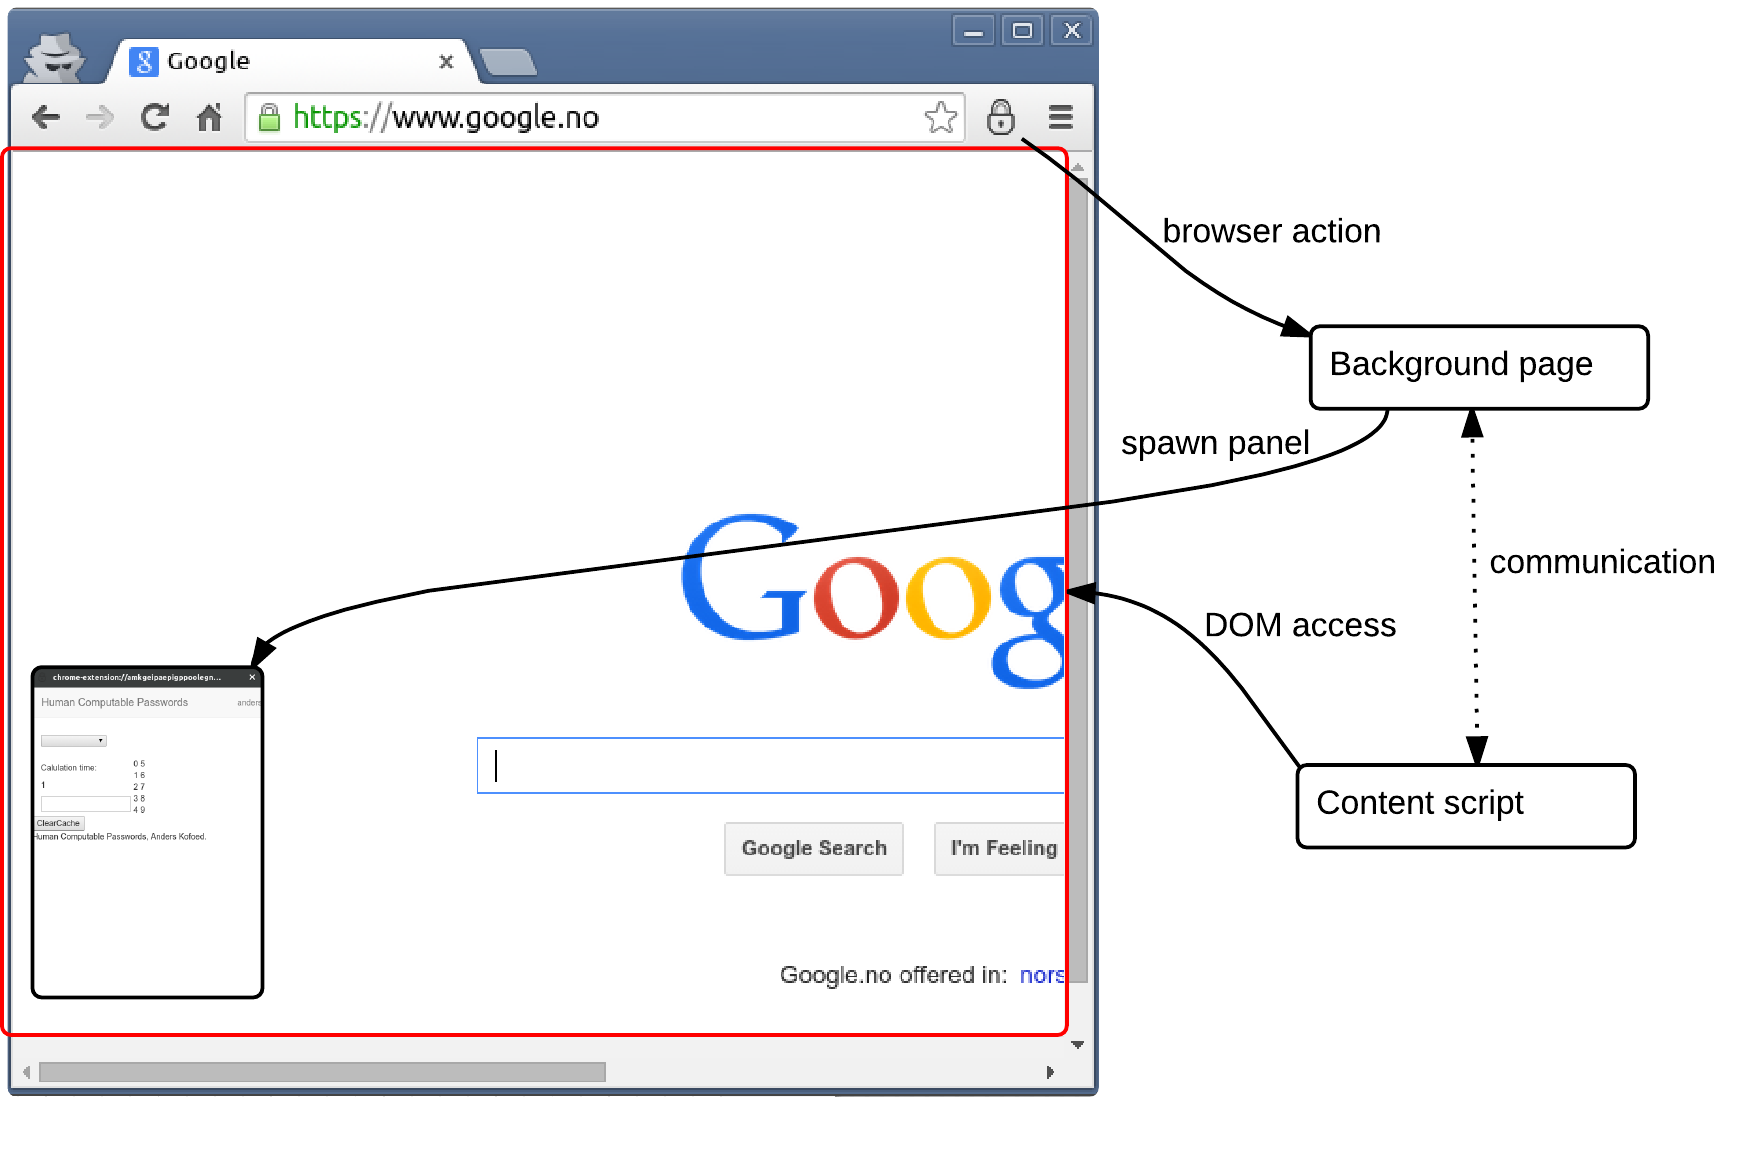
\includegraphics[width=\textwidth]{chrome-extension-ux} }
    \caption{Chrome extensions browser action and content scripts.}
    \label{extension-ux}
\end{figure}

\paragraph{Process isolation} are a set of mechanisms shielding the component from each other and from the web. Usually when javascript is loaded from the web the authority of the script is limited to the origin from where the script is loaded \cite{protecting-browsers}. Since the scripts used by the extensions is loaded from the file system, it does not have a origin in the same sense, and thus needs to be assigned one. This is done by including a public key in the url of the extension, allowing a packaged extensions to sign itself, freeing it from any naming authority or similar. The public key also enables usage of persistent data storage, since the origin of the extension can stay the same throughout updates and patches. This wouldn't be possible otherwise since the chrome local storage API relies on origin.
\par The different components also run in different processes. The content scripts are injected and ran in the same process as the active web page, while the core run in its own process started when the extension is initiated. \todo{paragraph not finished. Cross-origin js and malicious web site operators.}
\par Finally content scripts are ran in a separate javascript environment isolating it from the possibly insecure environment of the web site. The environment of the content scripts are called isolated world, which in practice is a separate set of javascript objects reflecting the ones of the underlying DOM of the web page. This means that the content script can read and edit the DOM of the page it is injected into, but not access variables or javascript functions present in the web page. Both the page and the content scripts sees no other javascript executing in their own isolated world, but they share the same DOM \cite{chrome-content-scripts}.

\par \autoref{extension-architecture} illustrates the architecture of chrome extensions with process isolation and isolated worlds.


%
%Instead of running the extensions with the same privileges as the browser, the extensions are ran using only a set of privileges specified before installing \cite{protecting-browsers}. The permissions are specified in a \emph{manifest.json} file, the "permissions" attribute contains the permissions specifying what the extensions will be allowed to do, the manifest file used in this project can be seen in \autoref{manifest}. Note that the only permission used is \emph{storage} which allows access to the chrome storage API. Next, extensions divides permissions between the different components, the content script has access to the content of the active page, and can send messages to the core. As the content script interacts with possibly insecure web pages and thus at risk of being attacked, they are low-privileged. With this division, a compromised content script does not pose a major risk to the core, unless the attacker manages to attack it through the secure messaging channel. The core has access to the extensions APIs, but only those specified in the manifest file as mentioned.
%
%\par In addition chrome extensions are limited  by three levels of isolation. The access to resources are limited to the origin of the extension, to be able to access another origin, typically the current active web page, the cross-origin permission has to be given. In the example manifest this permission is used to allow execution of the file \emph{content\_script} on all urls. In other cases this would be more restrictive, only allowing access to the least amount of origins. The second level of isolation isolates the processes of the content script and the extensions core, with each running in an isolated process. Finally the content script run in a separate javascript environment, an \emph{isolated world}, shielding it from the untrusted content of the active web page. This is meant to protect the extension from web attacks using malicious javascript. The architecture is illustrated in \autoref{extension-architecture} 
%




\begin{figure}[h]
   \fbox{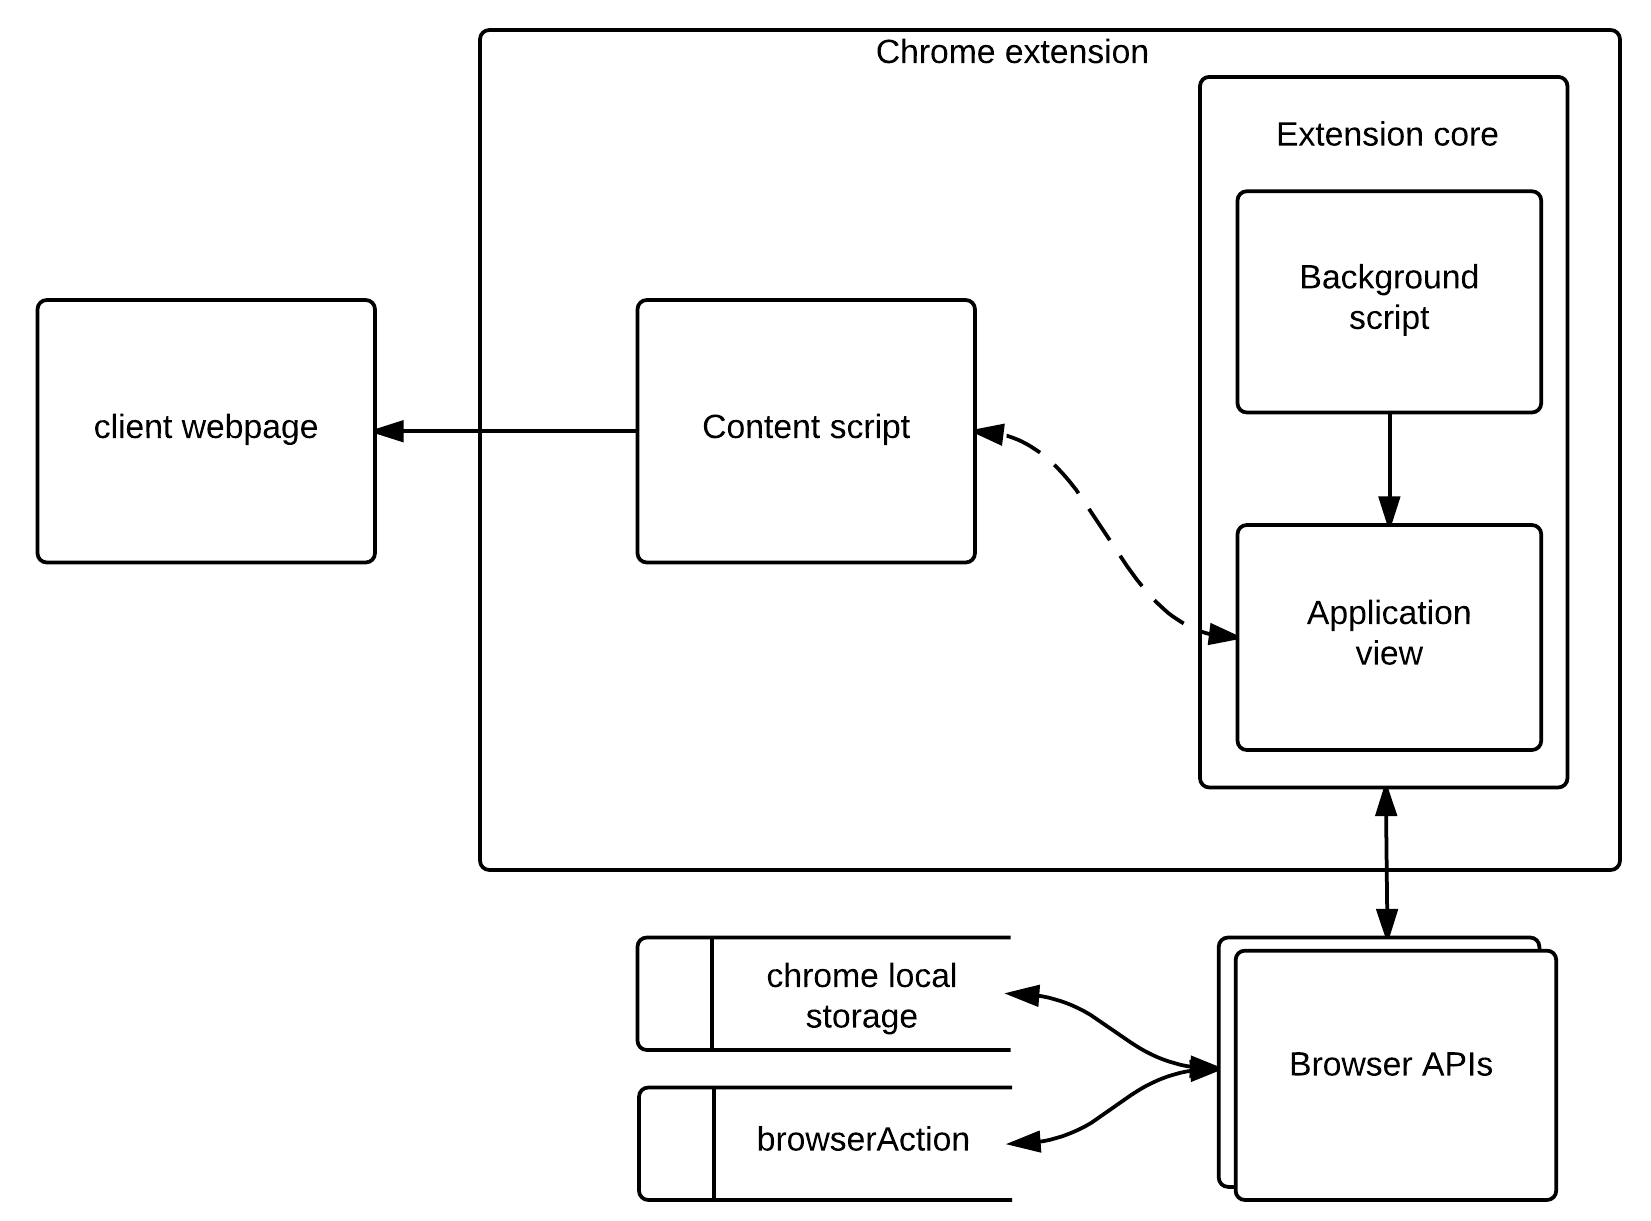
\includegraphics[width=\textwidth]{chrome-extension-architecture} }
    \caption{Chrome extension architecture.}
    \label{extension-architecture}
\end{figure}






\section{Usability Model}



\section{Security Model}




